\documentclass[10pt]{article}

%%%%%%%%%%%%%%%%%%%%%%%%%%%%%%%%%%%%%%%%%%%%%%%%%%%%%%%%%%%%%%%%%%%%%%%%%%%%%%%%
% LaTeX Imports
%%%%%%%%%%%%%%%%%%%%%%%%%%%%%%%%%%%%%%%%%%%%%%%%%%%%%%%%%%%%%%%%%%%%%%%%%%%%%%%%
\usepackage{amsfonts}                                                   % Math fonts
\usepackage{amsmath}                                                    % Math formatting
\usepackage{amssymb}                                                    % Math formatting
\usepackage{amsthm}                                                     % Math Theorems
\usepackage{arydshln}                                                   % Dashed hlines
\usepackage{attachfile}                                                 % AttachFiles
\usepackage{cancel}                                                     % Cancelled math
\usepackage{caption}                                                    % Figure captioning
\usepackage{color}                                                      % Nice Colors
\input{./lib/dragon.inp}                                                % Tikz dragon curve
\usepackage[ampersand]{easylist}                                        % Easy lists
\usepackage{fancyhdr}                                                   % Fancy Header
\usepackage[T1]{fontenc}                                                % Specific font-encoding
%\usepackage[margin=1in, marginparwidth=2cm, marginparsep=2cm]{geometry} % Margins
\usepackage{graphicx}                                                   % Include images
\usepackage{hyperref}                                                   % Referencing
\usepackage[none]{hyphenat}                                             % Don't allow hyphenation
\usepackage{lipsum}                                                     % Lorem Ipsum Dummy Text
\usepackage{listings}                                                   % Code display
\usepackage{marginnote}                                                 % Notes in the margin
\usepackage{microtype}                                                  % Niceness
\usepackage{lib/minted}                                                 % Code display
\usepackage{multirow}                                                   % Multirow tables
\usepackage{pdfpages}                                                   % Include pdfs
\usepackage{pgfplots}                                                   % Create Pictures
\usepackage{rotating}                                                   % Figure rotation
\usepackage{setspace}                                                   % Allow double spacing
\usepackage{subcaption}                                                 % Figure captioning
\usepackage{tikz}                                                       % Create Pictures
\usepackage{tocloft}                                                    % List of Equations
%%%%%%%%%%%%%%%%%%%%%%%%%%%%%%%%%%%%%%%%%%%%%%%%%%%%%%%%%%%%%%%%%%%%%%%%%%%%%%%%
% Package Setup
%%%%%%%%%%%%%%%%%%%%%%%%%%%%%%%%%%%%%%%%%%%%%%%%%%%%%%%%%%%%%%%%%%%%%%%%%%%%%%%%
\hypersetup{%                                                           % Setup linking
    colorlinks=true,
    linkcolor=black,
    citecolor=black,
    filecolor=black,
    urlcolor=black,
}
\RequirePackage[l2tabu, orthodox]{nag}                                  % Nag about bad syntax
\renewcommand*\thesection{\arabic{section} }                             % Reset numbering
\renewcommand{\theFancyVerbLine}{ {\arabic{FancyVerbLine} } }              % Needed for code display
\renewcommand{\footrulewidth}{0.4pt}                                    % Footer hline
\setcounter{secnumdepth}{3}                                             % Include subsubsections in numbering
\setcounter{tocdepth}{3}                                                % Include subsubsections in toc
%%%%%%%%%%%%%%%%%%%%%%%%%%%%%%%%%%%%%%%%%%%%%%%%%%%%%%%%%%%%%%%%%%%%%%%%%%%%%%%%
% Custom commands
%%%%%%%%%%%%%%%%%%%%%%%%%%%%%%%%%%%%%%%%%%%%%%%%%%%%%%%%%%%%%%%%%%%%%%%%%%%%%%%%
\newcommand{\nvec}[1]{\left\langle #1 \right\rangle}                    %  Easy to use vector
\newcommand{\ma}[0]{\mathbf{A} }                                         %  Easy to use vector
\newcommand{\mb}[0]{\mathbf{B} }                                         %  Easy to use vector
\newcommand{\abs}[1]{\left\lvert #1 \right\rvert}                       %  Easy to use abs
\newcommand{\pren}[1]{\left( #1 \right)}                                %  Big parens
\let\oldvec\vec
\renewcommand{\vec}[1]{\oldvec{\mathbf{#1} } }                            %  Vector Styling
\newtheorem{thm}{Theorem}                                               %  Define the theorem name
\newtheorem{definition}{Definition}                                     %  Define the definition name
\definecolor{bg}{rgb}{0.95,0.95,0.95}
\newcommand{\java}[4]{\vspace{10pt}\inputminted[firstline=#2,
                                 lastline=#3,
                                 firstnumber=#2,
                                 gobble=#4,
                                 frame=single,
                                 label=#1,
                                 bgcolor=bg,
                                 linenos]{java}{#1} }
\newcommand{\python}[4]{\vspace{10pt}\inputminted[firstline=#2,
                                 lastline=#3,
                                 firstnumber=#2,
                                 gobble=#4,
                                 frame=single,
                                 label=#1,
                                 bgcolor=bg,
                                 linenos]{python}{#1} }
\newcommand{\js}[4]{\vspace{10pt}\inputminted[firstline=#2,
                                 lastline=#3,
                                 firstnumber=#2,
                                 gobble=#4,
                                 frame=single,
                                 label=#1,
                                 bgcolor=bg,
                                 linenos]{js}{#1} }
%%%%%%%%%%%%%%%%%%%%%%%%%%%%%%%%%%%%%%%%%%%%%%%%%%%%%%%%%%%%%%%%%%%%%%%%%%%%%%%%
% Beginning of document items - headers, title, toc, etc...
%%%%%%%%%%%%%%%%%%%%%%%%%%%%%%%%%%%%%%%%%%%%%%%%%%%%%%%%%%%%%%%%%%%%%%%%%%%%%%%%
\pagestyle{fancy}                                                       %  Establishes that the headers will be defined
\fancyhead[LE,LO]{Computer Systems Notes}                                  %  Adds header to left
\fancyhead[RE,RO]{Zoe Farmer}                                       %  Adds header to right
\cfoot{ \thepage }
\lfoot{CSCI 2400}
\rfoot{Han}
\title{Computer Systems Notes}
\author{Zoe Farmer}

%%%%%%%%%%%%%%%%%%%%%%%%%%%%%%%%%%%%%%%%%%%%%%%%%%%%%%%%%%%%%%%%%%%%%%%%%%%%%%%%
% Beginning of document items - headers, title, toc, etc...
%%%%%%%%%%%%%%%%%%%%%%%%%%%%%%%%%%%%%%%%%%%%%%%%%%%%%%%%%%%%%%%%%%%%%%%%%%%%%%%%
\pagestyle{fancy}                                                 %  Establishes that the headers will be defined
\fancyhead[LE,LO]{Problem Set 5}                                  %  Adds header to left
\fancyhead[RE,RO]{Zoe Farmer, Jeremy Granger, Ryan Roden}     %  Adds header to right
\cfoot{\mlptikz[size=0.25in, text=on, textposx=0, textposy=0, textvalue=\thepage, textscale=0.75in]{applejack} }
\lfoot{CSCI 3104}
\rfoot{Clauset}
\title{Problem Set Five}
\author{Zoe Farmer\\Jeremy Granger\\Ryan Roden}
%%%%%%%%%%%%%%%%%%%%%%%%%%%%%%%%%%%%%%%%%%%%%%%%%%%%%%%%%%%%%%%%%%%%%%%%%%%%%%%%
% Beginning of document items - headers, title, toc, etc...
%%%%%%%%%%%%%%%%%%%%%%%%%%%%%%%%%%%%%%%%%%%%%%%%%%%%%%%%%%%%%%%%%%%%%%%%%%%%%%%%
\begin{document}

\maketitle

\begin{easylist}[enumerate]
    @ Implement Huffman's algorithm from scratch using a priority queue data structure. You may not use any library that
    implements a priority queue (or equivalent) data structure-the point here is to implement it yourself, using only
    basic language features. Within the priority queue, ties should be broken uniformly at random.\newline

    Your implementation should take as input a string $x$ of ASCII characters, perform the Huffman encoding, and then
    output the following: (i) the ``codebook'' which is a table containing each of the symbols in $x$ and its corresponding
    binary Huffman encoding and (ii) the encoded string $y$.\newline

    Submit your code implementing Huffman. Be sure to include code comments.
    @ The data file on the class website for PS5 contains the text of a famous poem by Robert Frost. The text comes in
    the form of a string $\sigma$ containing $l = 761$ symbols drawn from an alphabet $\Sigma$ with $|\Sigma| = 31$
    symbols (24 alphabetical characters, 6 punctuation marks and 1 space character).
    @@ A plaintext ASCII character normally takes 8 bits of space. How many bits does $\sigma$ require when encoded in
    ASCII?
    @@@ This is simply $ 8 \cdot l= 6088$.
    @@ The theoretical lower limit for encoding is given by the entropy of the frequency of the symbols in the string:
        \[ H = - \sum^{|\Sigma|}_{i=1} \left( \frac{f_i}{l} \right) \log_2 \left( \frac{f_i}{l} \right) \]
        where $f_i$ is the frequency of the $i$th symbol of the alphabet $\Sigma$. Because we take $\log_2$, $H$ has
        units of ``bits.'' What is the theoretical lower limit for the number of bits required to encode $\sigma$?
    @@@ This can be restated with variables filled, and subsequently solved with a python one-liner.

        \[
            H = - \sum^{31}_{i=1} \left( \frac{f_i}{761} \right) \log_2 \left( \frac{f_i}{761} \right) = 4.12543135174
        \]

        \begin{pythoncode*}{gobble=12, xleftmargin=1in}
            Hsum = -1 * sum([((alpha[f] / length) *
                            numpy.log2(alpha[f] / length))
                            for f in alpha])
        \end{pythoncode*}

    @@ Encode $\sigma$ using your Huffman encoder and report the number of bits in the encoded string. Comment on this
    number relative to your theoretical calculation from part (b).
    @@@ Using our encoder this is 2323 bits.
    @@ How many additional bits would be required to write down the codebook? Could this number be made any smaller?
    @@@ Assuming 8 bits per character and 4 bits per integer value, we'd need 384 bits with the following code.

        \[ \begin{aligned}
            \{'r': 2,&    'a': 3,&    ',': 30,&  ';': 172,&  ':': 173,& 'y': 28,&  'n': 12,& 'w': 30,&\\
              'v': 21,&   'u': 29,&   't': 4,&   's': 3,&    '-': 253,& 'q': 255,& 'p': 62,& 'o': 6,&\\
              '.': 87,&   'm': 42,&   'l': 11,&  'k': 20,&   'j': 254,& 'i': 4,&   'h': 14,& 'g': 20,&\\
              'f': 62,&   'e': 0,&    'd': 13,&  'c': 63,&   'b': 11,&  '!': 252,& '\quad': 2\}
        \end{aligned} \]

    @ Using your Huffman implementation from question 1, conduct the following numerical experiment.\newline

    Show via a plot on log-log axes that the asymptotic running time of your Huffman encoder is $O(n \log n)$, where $n
    = |\Sigma|$ is the size of the input alphabet $\Sigma$. The deliverable here is a single figure (like the one below)
    showing how the number of atomic operations $T$ grows as a function of $n$. Include two trend lines of the form $c
    \times n \log n$ that bound your results from above and below. Label your axes and trend line. Include a clear and
    concise description (1-2 paragraphs) of exactly how you ran your experiment.

    @@ Once we have a workable Huffman Encoder, we can now run trials to determine its runtime complexity. We add an
    {\ttfamily operations} class variable to our encoder, and then account for every elementary operation that takes
    place. Using Python3's extended unicode support we can generate large frequency dictionaries quickly that still have
    meaning. The below code when given the desired length of our frequency dictionary will create a randomized
    dictionary of unicode characters and their ``frequencies''.

        \begin{pythoncode*}{gobble=12, xleftmargin=1in}
            def generate_alpha(length):
                ''' Generates random frequency dict '''
                alpha = {}
                for i in range(length):
                    alpha[chr(32 + i)] = random.randint(0, 100)
                return alpha
        \end{pythoncode*}

    In order to successfully complete the trials we then wrap this in another {\ttfamily for}-loop which checks runtime
    complexity at logarithmic intervals.

        \begin{pythoncode*}{gobble=12, xleftmargin=1in}
            n  = []  # Lengths
            op = []  # Operation count
            for length in [2**x for x in range(1, 14)]:
                huffman = Huffman()
                # Our alphabet generator from before
                alpha = generate_alpha(length)
                # Create the encoder with our alphabet
                huffman.create_code(alpha)
                # X-value: number of elements in alphabet
                n.append(length)
                # Y-value: number of operations required
                op.append(huffman.operations)
        \end{pythoncode*}

    We then use {\ttfamily matplotlib.pyplot} to create a graph of our results. Please see figure~\ref{fig:complex}.
    Note, it is highly recommended to examine the source code written. Any questions you have about the code itself will
    most likely be answered by either the code or the comments.

        \begin{figure}[!ht]
            \centering
            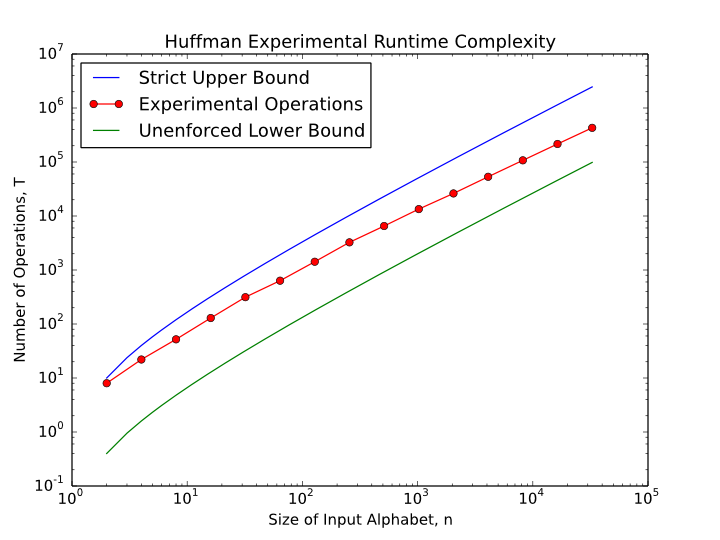
\includegraphics[scale=0.75]{./img/complexity.png}
            \caption{Runtime Complexity of Huffman Encoding}
            \label{fig:complex}
        \end{figure}

    @ You and Gollum are having a competition to see who can compute the $n$th Fibonacci number more quickly. Gollum
    asserts the classic recursive algorithm:

        \begin{pythoncode*}{gobble=12, xleftmargin=0.5in}
            def Fib(n):
                if n < 2:
                    return n
                else:
                    return Fib(n-1) + Fib(n-2)
        \end{pythoncode*}

    which he claims takes $R(n) = R(n - 1) + R(n - 2) + c = O(\Phi^n)$ time and space.\newline

    You counter with a dynamic programming algorithm, which you claim is asymptotically faster. Recall that dynamic
    programming is a kind of recursive strategy in which instead of simply dividing a problem of size $n$ into two
    smaller problems whose solutions can be merged, we instead construct a solution of size $n$ by merging smaller
    solutions, starting with the base cases. The difference is that in this ``bottom up'' approach, we can reuse
    solutions to smaller problems without having to recompute them.
    @@ You suggest that by ``memoizing'' (a.k.a.\ memorizing) the intermediate Fibonacci numbers, by storing them in an
    array $F[n]$, larger Fibonacci numbers can be computed more quickly. You assert the following algorithm.

        \begin{pythoncode*}{gobble=12, xleftmargin=0.7in}
            def MemFib(n):
                if n < 2:
                    return n
                else:
                    if F[n] is None:
                        F[n] = MemFib(n-1) + MemFib(n-2)
                    return F[n]
        \end{pythoncode*}

    @@@ Describe the behavior of MemFib(n) in terms of a traversal of a computation tree. Describe how the array F is
    filled.
    @@@@ MemFib will always see MemFib($n-1$) as the element that needs to be determined until $n - 1 < 2$, at which
    point it will merely return $n$. This means that when MemFib($n - 2$) is executed, the algorithm will just pull the
    value from the filled array, and not traverse that branch. This essentially means that \textit{only} the left
    branches of the recursion tree are executed until we reach the base case. This also means that $F$ is filled from
    index 2 to index $n$. To see the computation tree, please reference Figure~\ref{fig:tree}, where only the left
    branches lead to recursion and all right branches are array indexing operations.

    \begin{figure}[!ht]
        \centering
        \scalebox{1}{%
        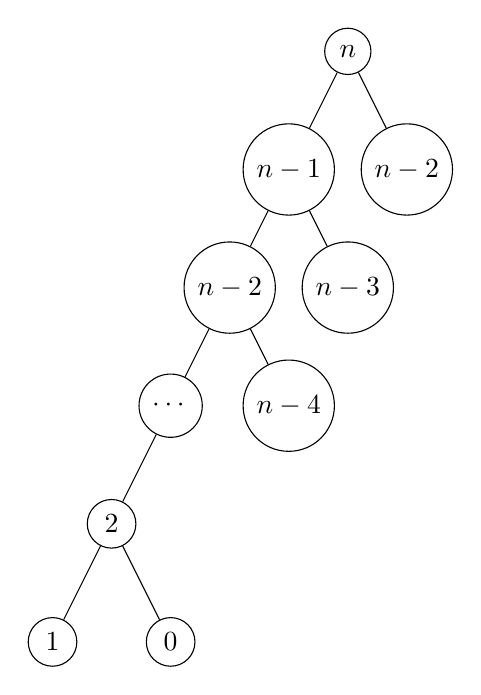
\begin{tikzpicture}
        \node[circle,draw](z){ $n$ }
            child{%
              node[circle,draw]{$n - 1$}
                child{%
                  node[circle,draw]{$n - 2$}
                  child{%
                    node[circle,draw]{$\cdots$}
                    child{%
                      node[circle,draw]{$2$}
                      child{%
                        node[circle,draw]{$1$}
                        child[missing]
                        child[missing]
                      }
                      child{%
                        node[circle,draw]{$0$}
                        child[missing]
                        child[missing]
                      }
                    }
                    child[missing]
                  }
                  child{%
                    node[circle,draw]{$n - 4$}
                    child[missing]
                    child[missing]
                  }
                }
                child{%
                  node[circle,draw]{$n - 3$}
                  child[missing]
                  child[missing]
                }
              }
            child{%
              node[circle,draw]{$n - 2$}
              child[missing]
              child[missing]
                };
        \end{tikzpicture}
        }
        \caption{Computation Tree}
        \label{fig:tree}
    \end{figure}

    @@@ Compute the asymptotic running time. Prove this result by induction.
    @@@@ The asymptotic running time of this algorithm is $O(n)$ due to its perfectly unbalanced recursion tree.

        \[ \begin{aligned}
            \text{Recurrence Relation of MemFib} &\to& M(n) = M(n) + M(1)\\
            \text{Index Cost} &\to& M(1) = O(1)\\
            \text{Assume} &\to& M(k) = k\\
            \text{Therefore} &\to& M(k) \Rightarrow M(k + 1)\\
            \text{Substituting} &\to& M(k + 1) \Rightarrow M(k + 1)\\
            \text{Therefore} &\to& M(n) = {O(n)}_\blacksquare
        \end{aligned} \]

    @@ Gollum then claims that he can beat your algorithm in both time and space by eliminating the recursion completely
    and building up directly to the final solution by filling the $F$ array in order. Gollum's new algorithm is

        \begin{pythoncode*}{gobble=12, xleftmargin=1in}
            def DynFib(n):
                F[0] = 0
                F[1] = 1
                for i in range(2, n):
                    F[i] = F[i-1] + F[i-2]
                return F[n]
        \end{pythoncode*}

    How much time and space does DynFib(n) take? Justify your claim and compare your answers to those of your solution
    in part (a).
    @@@ Using Gollum's new algorithm we see that it is very similar to the previous one. In fact, Gollum's algorithm is
    no more time efficient than the original, and they both run in $O(n)$ time. They also have the same space
    requirements, however the difference between the two is the fact that MemFib makes recursive calls, which add to the
    memory requirements in the stack, while DynFib avoids this through application of a {\ttfamily for}-loop. Thus we
    can establish that the space complexity of MemFib is $O(2n)$ and DynFib is $O(n)$, which when measured
    asymptotically we see that both are $O(n)$.

    @@ With a gleam in your eye, you tell Gollum that you can do it even more efficiently because you do not, in fact,
    need to store all the intermediate results.  Over Gollum's pathetic cries, you say

        \begin{pythoncode*}{gobble=12, xleftmargin=1in}
            def FasterFib(n):
                a = 0
                b = 1
                for i in range(2, n):
                    c = a + b
                    a = b
                    b = c
                return b
        \end{pythoncode*}

    Derive the time and space requirements for FasterFib(n). Justify your claims.
    @@@ Again, FasterFib runs no faster than the other two, it just uses far less space. It still has to iterate through
    $n$ values, but it only keeps the values that it needs for the next calculation. This means that it's runtime
    complexity is $O(n)$, but the space complexity drops to $O(1)$.

    @@ Give a table that lists each of the four algorithms, its asymptotic time and space requirements, and the implied
    or explicit data structures each requires.  Briefly compare and contrast the algorithms in these terms.
    @@@ Please reference Table~\ref{table:algorithms}

    \begin{table}[!ht]
        \centering
        \begin{tabular}{|l|lll|}
            \hline
            Algorithm & Time Complexity & Space Complexity & Data Structures\\
            \hline
            Fib       & $O(\Phi^n)$ & $O(\Phi^n)$ & Binary Recursion Tree\\
            MemFib    & $O(n)$ & $O(n)$ & Binary Recursion Tree/Array\\
            DynFib    & $O(n)$ & $O(n)$ & Array\\
            FasterFib & $O(n)$ & $O(1)$ & Variables\\
            \hline
        \end{tabular}
        \caption{Algorithm's Complexity}
        \label{table:algorithms}
    \end{table}

    @ Gollum hands you a set $X$ of $n > 0$ intervals on the real line and demands that you find a subset of these
    intervals $Y \subset X$, called a tiling cover, where the intervals in $Y$ cover the intervals in $X$, that is,
    every real value contained within some interval in X is contained in some interval $Y$. The size of a tiling cover
    is just the number of intervals. To satisfy Gollum, you must return the minimum cover $Y_{min}$ : the tiling cover
    with the smallest possible size.\newline

    For the following, assume that Gollum gives you an input consisting of two arrays $X_L [1, \ldots, n]$ and $X_R [1
    \ldots n]$, representing the left and right endpoints of the intervals in $X$.
    @@ Describe in words and give pseudo-code for a greedy algorithm to compute the smallest $Y$ in $O(n \log n)$ time.
    @@@ This algorithm first formats the intervals into a sorted array of tuples that have the same start point. Once
    this has been completed we iterate through the array in sorted order, taking the longest interval gain in each and
    adding it to our cover. This establishes a cover that takes only the largest gain and uses it to extend the gain
    further, as it then ignores any new interval with starting value less than the ending value of our previous.

    This is $O(n \log(n))$ as it iterates through the array only once, yielding $O(n)$, and at each step it performs
    $O(\log(n))$ operations, yielding $O(n \log(n))$.

        \begin{pythoncode*}{gobble=12, xleftmargin=1in}
            def main():
                xl = [0, 1, 2, 3, 4, 1, 5]
                xr = [1, 4, 3, 8, 5, 3, 13]

                zipped = list(zip(xl, xr))
                raw_sets = sorted(zipped, key=lambda pair: pair[0])

                sets = []
                for item in raw_sets:
                    start = item[0]
                    group = [item]
                    for n in raw_sets:
                        if n[0] == start and n != item:
                            group.append(n)
                            raw_sets.pop(raw_sets.index(n))
                    sets.append(group)

                print(sets)

                cover = []
                previous = sets[0][0]
                for item in sets:
                    if item[0][0] < previous[1]:
                        pass
                    longest = None
                    for pair in item:
                        length = pair[1] - pair[0]
                        if previous:
                            length = pair[1] - previous[1]
                        if longest is None:
                            longest = pair
                        elif length > (longest[1] - longest[0]):
                            longest = pair
                    cover.append((longest[0], longest[1]))
                    previous = (longest[0], longest[1])
                print(cover)
        \end{pythoncode*}

    @@ Prove that this algorithm (i) covers each component and (ii) produces the minimal cover for each component.
    Explain why these conditions are necessary and sufficient for the correctness of the algorithm.
    @@@ This algorithm must cover each component in the interval as it traverses the entire array once, and since it
    takes only the greedy choice, it also produces the minimal cover.
\end{easylist}

\end{document}
